% !TeX root = ../thesis.tex
\section{Background}
The background section will cover four topics.
First the mathematics employed in this project will be covered. 
This consists of Thiele's differential equation and the fourth-order Runge-Kutta method for solving differential equations.
This is followed by general information on parallelization and the potential benefits of using the GPU compared to the CPU.
After this the CUDA platform, CUDA C and F\# with Alea.cuBase will be presented.


\subsection{Thiele's differential equation and the Runge-Kutta Method}
The goal of the computations done in this thesis is to estimate the amount of money (reserve) required to be able to fulfil the obligations of a given insurance plan.
Thiele's differential equation\cite{thiele} called ``the fundament of modern life insurance mathematics''\cite{thiele:quote} is a tool for determining conditional expected values in intensity-driven Markov processes.
It can be used to express a variety of life insurance products as long as they can be described by multi-state Markov processes.
The equation is expressed below in equation \ref{eq:thiele}. It consists of the following parts:

\begin{itemize}
\item $V_t$ is the reserve at time $t$
\item $\pi_t$ is the premium paid at time $t$
\item $b_t$ is the benefit paid by the insurer at time $t$
\item $\mu_{x+t}$ is the mortality intensity at time $t$ with a person of age age $x$ at the time of signing the contract
\item $r_t$ is interest-rate at time $t$
\end{itemize}

\begin{equation}\label{eq:thiele}
\frac{d}{dt}V_t = \pi_t - b_t \mu_{x+t} + (r_t + \mu_{x+t}) V_t
\end{equation}

With a differential equation such as this, we need a way to solve it. 
The Runge-Kutta method\cite{runge-kutta} is a method for integrating ordinary differential equations by using a trial step at the midpoint of an interval to cancel out lower-order error terms.
The fourth-order version of the method can be seen below in equation \ref{eq:rk4}.

\begin{equation}\begin{aligned}\label{eq:rk4}
&k_1 = h f(x_n, y_n)\\
&k_2 = h f(x_n + \frac{1}{2}h, y_n + \frac{1}{2}k_1)\\
&k_3 = h f(x_n + \frac{1}{2}h, y_n + \frac{1}{2}k_2)\\
&k_4 = h f(x_n + h, y_n + k_3)\\
&y_{n+1} = y_n + \frac{1}{6}k_1 + \frac{1}{3}k_2 + \frac{1}{3}k_3 + \frac{1}{6}k_4 + O(h^5)
\end{aligned}\end{equation}

\subsection{Parallelization and the GPU}
Parallelization is the act of taking one large task and splitting it into smaller tasks that run concurrently (''in parallel'').
This could for example be an algorithm that initially does some computation that loops $n$ times where each iteration is independent and takes $w$ time to complete, but is altered to instead utilize $n$ tasks that each execute one iteration's worth of work.
Instead of taking $w \cdot n$ time time, it can now be done in just $w$ time plus whatever overhead is associated with creating the tasks and dividing the work.
This is reliant on each iteration being independent, as if the iterations are dependent on each-other then it can not be executed before the previous iteration completes.
Loops isn't the only way to utilize parallelization and all independent tasks can in theory be parallelized. 
Utilizing various synchronization techniques, partially dependent calculations can also harness the power of parallelization, though at the risk of increased complexity and deadlocks.
As only independent computation parallelization is utilized, other forms will not be discussed further.

Parallelization can be performed on multi-core CPUs utilizing constructs such as processes and threads, but can especially be utilized by GPUs that were designed for compute-intensive and highly parallel computations, precisely what graphics rendering is about.
This is because unlike the CPU which is specialized for data-caching and flow control, the GPU has more transistors dedicated to data processing as illustrated by figure \ref{cpugpu}. \textbf{TODO - image by CUDA C Programming guide - credit or remake}

\begin{figure}[h!]
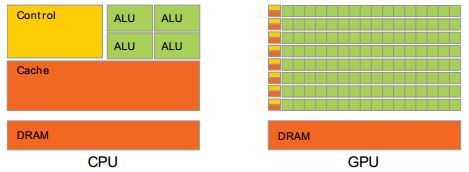
\includegraphics{cpugpu.jpg}
\caption{The GPU devotes more transistors to data processing\cite{cuda_c_programming_guide}\label{cpugpu}}
\end{figure}

%http://docs.nvidia.com/cuda/pdf/CUDA_C_Programming_Guide.pdf
%highly parallel, multithreaded, manycore processor with tremendous computational horsepower and very high memory bandwidth
%The reason behind the discrepancy in floating-point capability between the CPU and the GPU is that the GPU is specialized for compute-intensive, highly parallel computation - exactly what graphics rendering is about - and therefore designed such that more transistors are devoted to data processing rather than data caching and flow control
%Talk about GPU vs CPU and parallelization in general

\subsection{CUDA and CUDA C}
CUDA is NVIDIAs parallel computing platform and programming model for harnessing the power of the GPU.
The CUDA platform consists of the CUDA C and C++ language (referred to as CUDA C from this point), based on C and C++ but with some alterations.
It also has parallel computing extensions for other languages such as Fortran and Python.
The CUDA Toolkit is also a part of the platform, which consists of a compiler, math libraries and tools for debugging and optimizing performance as well as guides, user manuals, API references and other documentation.

\subsubsection{CUDA Architecture}
The CUDA model is build around a hierarichal architecture of the GPU. 
At the top of the architecture is the streaming multi-processor (SM) of which a GPU can have many. 
Each SM consists of multiple CUDA cores that are used to concurrently execute a group of 32 threads known as a warp. As the SM executes the instructions in terms of warps, the total amount of threads in a block should be a multiple of the warp-size for maximum efficiency.
Each SM executes one group of threads that have access to a shared memory-space. This group of threads, which should be a multiple of warps, is called a block. 
As each SM executes a block at a time, more SMs available to the GPU will speed up the execution of the total amount of blocks. 
This also means that the amount of blocks should be a multiple of the amount of multiprocessors for maximum efficiency. %confirm

\subsubsection{Memory}
A thread has access to memory only available to itself using registers as long as they're available and falling back on local memory otherwise.
Beyond that it has access to shared memory that is available to all threads in the same block as well as global memory accessible to all threads in all blocks.
There is also constant memory and texture memory both of which are fast but immutable. 
There is also a L1 and L2 cache \textbf{todo.. used for global/local memory I suppose?}.
The properties of the various memory types can be seen in table \ref{table:memorytypes}.
{\renewcommand{\arraystretch}{3}%
\begin{table}[h!]
\centering
\begin{tabular}{ | c | c | c | c | }
  \hline
           & Mutable & Speed & Cached \\ \hline
  Register & Yes     & Fast  & No     \\ \hline
  Local    & Yes     & Slow  & Yes    \\ \hline
  Shared   & Yes     & Fast  & No     \\ \hline
  Global   & Yes     & Slow  & Yes    \\ \hline
  Texture  & No      & Fast  & Yes    \\ \hline
  Constant & No      & Slow  & Yes    \\ \hline

\end{tabular}
\caption{Properties of CUDA memory types\label{table:memorytypes}}
\end{table}

Talk about memory throughput

\subsubsection{CUDA C}
CUDA C is mostly C with added declaration specifiers for methods and variables. The most essential declaration specifier is the \textbf{\_\_global\_\_} specifier which declares a method to be a \textbf{kernel}. Kernels are void-methods that are callable from the CPU but will be executed on the GPU. Code sample \ref{cuda_add} shows a simple kernel performing vector addition of the vectors of size $N$.

\begin{lstlisting}[language=C++, caption=CUDA C addition kernel, label=cuda_add]
__global__ void Add(float* a, float* b, float* result){
	//unique id within the kernel
	int i = threadIdx.x + blockIdx.x * blockDim.x;
	// (blockIdx always 0 in this example)
	result[i] = a[i] + b[i];
}

int main(){
	...//Initiate memory on host and device
	Add<<<1, N>>>(a, b, result); //invoke kernel on 1 block of N threads
	...//Copy back results, free memory as appropriate
}
\end{lstlisting}

Another thing to note is the launch-parameters of the kernel which specify the amount of blocks and the amount of threads per block. A block can be organized into either one-dimensional, two-dimensional or three-dimensional grids. This is convenient in the case of working with for example matrices, but is not utilized in this thesis and will not be covered in further detail.

CUDA C also has other declaration specifiers. \textbf{\_\_device\_\_} specifies that a method will only be compiled for the GPU (which can be referenced by kernels), \textbf{\_\_host\_\_} specifies that a method will be available for the CPU. These two specifiers can also be used together for compilation to both platforms.
Variables have the \textbf{\_\_device\_\_} qualifier, as well as \textbf{\_\_constant\_\_} to indicate it should be stored in constant memory or \textbf{\_\_shared\_\_} for shared memory.

As it is based on C, dynamic memory must be allocated using $malloc$ and subsequently de-allocated by $free$.
This operation also has to be done for the device memory using the equivalent $cudaMalloc$ and $cudaFree$.
The tediousness of this is one of the many benefits from using a more modern language, but at the cost of control that could potentially decrease performance.

\subsection{F\# and Alea.cuBase}
F\#\cite{fsharp} is an open source, cross-platform functional programming language originating from Microsoft that runs on the .NET platform.
Alea.cuBase by QuantAlea\cite{quantalea} is a commercial language-integrated compiler for F\# that allows for CUDA development on the .NET platform.
By relying on run-time code-generation it allows for extremely extensible kernels to an extend not easily possible in CUDA C.

It utilizes F\#'s meta-programming support Code Quotation\cite{ms:quotations} for automatic run-time generation of abstract syntax-trees that are then compiled into CUDA's Instruction Set Architecture (ISA) Parallel Thread Execution (PTX) code using Alea.cuBase's compilation API.
Code sample \ref{cubase_add} shows what a simple squaring-kernel could look like in Alea.cuBase F\#. 

\begin{lstlisting}[caption=Alea.cuBase square kernel, label=cubase_add]
let Square = cuda { //use the Alea.cuBase cuda workflow
  let! kernel = <@ fun (a:deviceptr<int>) (result:deviceptr<int>) ->
      let i = blockIdx.x * blockDim.x + threadIdx.x
      result.[i] <- a.[i] * a.[i] @> |> Compiler.DefineKernel
  //<@ @> is the Code Quotation, that is then compiled with Alea.cuBase
  return Entry(fun program ->
    let worker = program.Worker
    let kernel = program.Apply kernel
    //return host-execution method
    fun (a:int[]) ->
      use a = worker.Malloc(a)
      use result = worker.Malloc(Array.zeroCreate a.Length)
      kernel.Launch (LaunchParam(1, a.Length)) a.Ptr result.Ptr
      result.Gather()) //return result
}
[<EntryPoint>]
let main argv = 
  let a = [| for i in 1 .. 10 -> i |]
  use program = Square |> Compiler.load Worker.Default
  program.Run a |> Array.iter (fun e -> printfn "%d" e)
  0 //return 0 to indicate success
\end{lstlisting}

The cuda workflow/computation expression (or "monad" for the so inclined) contains the kernel defined with Code Quotations and compiled to an actual kernel and returns a host-side execution method that will handle allocation and de-allocation of device-side memory. 
As we are using F\#, the deallocation can be handled automatically by using the $use$-keyword. 
The program is then loaded to a worker (a CUDA context and background-thread) in the main method compiling the PTX to NVIDIA internal ISA.
The program is then run using the parameters defined in the run-time method of the cuda workflow (in this case, it just takes an integer array) and the result is returned to the CPU where it can be processed (in this example, the result is simply printed).

\subsection{Hardware}
As the intended audience for this particular application of parallelization is fairly limited and can be expected to afford specific hardware, it has not been a concern that specific hardware may be required to run it.
The minimal requirement to run the program is a GPU of at least compute capability 2.0.
The code was only tested on the NVIDIA Tesla C2075 GPU which has the following properties:

\begin{itemize}
\item Compute capability: 2.0
\item Multiprocessors: 14
\item CUDA cores per Multiprocessor: 32
\item Clock rate: 1147 MHz (1.15 GHz)
\item Memory clock rate: 1566 MHz
\item Total global memory: 17592186044416 MBytes
\item Total constant memory: 65536 bytes
\item Total shared memory per block: 49152 bytes
\item Total amount of registers per block: 32768
\item Total amount of threads per multiprocessor: 1536
\item Total amount of threads per block: 1024
\item L2 Cache Size: 786432 bytes
\item Warp size: 32
\item Maximum sizes of each dimension of a block: 1024 x 1024 x 64
\item Maximum sizes of each dimension of a grid: 65535 x 65535 x 65535
\item Texture alignment: 512 bytes
\item Maximum memory pitch: 2147483647 bytes
\item Concurrent copy and kernel execution: Yes with 2 copy engines
\item Run time limit on kernels: No
\item Integrated GPU shareing Host Memory: No
\item Support host page-locked memory mapping: Yes
\item Concurrent kernel execution: Yes
\end{itemize}